\documentclass[../../main.tex]{subfiles}
\begin{document}

\begin{flushright}
  \footnotesize\textit{【自動文字起こし・要確認】}
\end{flushright}

{\bf [解答]} 題意の放物線は
\begin{align}
  y = f(x) = \dfrac{m}{a^2}x(2a-x)
\end{align}
である．
\begin{align}
  S_m &= \int_0^{2a} f(x) dx \\
  &= \dfrac{1}{6} \dfrac{m}{a^2} (2a)^3 = \dfrac{4}{3}ma \quad \cdots \text{①}
\end{align}

\begin{figure}[htb]
  \centering
  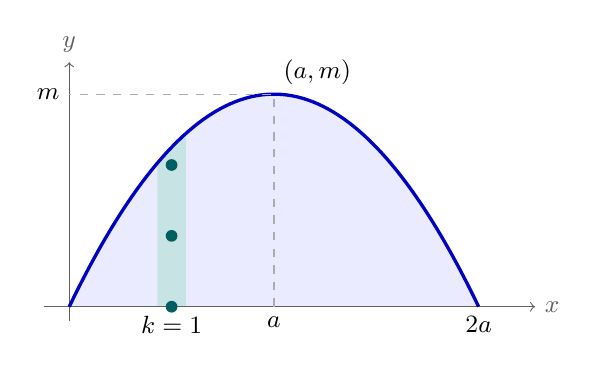
\begin{tikzpicture}[x=1.3cm,y=0.9cm,every node/.style={font=\small}]
    % a=2, m=3 とした格子点の配置例．
    \fill[blue!8] (0,0)--plot[domain=0:4,samples=80]
    (\x,{0.75*\x*(4-\x)})--cycle;
    \fill[teal!22] (0.86,0)--plot[domain=0.86:1.14,samples=30]
    (\x,{0.75*\x*(4-\x)})--(1.14,0)--cycle;
    \draw[->,gray!75!black] (-0.25,0)--(4.55,0) node[right] {$x$};
    \draw[->,gray!75!black] (0,-0.2)--(0,3.45) node[above] {$y$};
    \draw[blue!75!black,very thick,domain=0:4,samples=80]
    plot (\x,{0.75*\x*(4-\x)});
    \draw[gray!65,dashed] (2,0)--(2,3)--(0,3);
    \foreach \j in {0,1,2} {
      \node[circle, fill=teal!75!black, inner sep=1.5pt] at (1,\j) {};
    }
    \node[left] at (0,3) {$m$};
    \node[below] at (1,0) {$k=1$};
    \node[below] at (2,0) {$a$};
    \node[below] at (4,0) {$2a$};
    \node[above right] at (2,3) {$(a,m)$};
  \end{tikzpicture}
  \caption{放物線下の領域と，$x=k$に並ぶ格子点の例}
\end{figure}

又，$L_m = \sum_{k=0}^{2a} \{ [f(k)] + 1 \}$ だから，$f(k)-1 < [f(k)] \le f(k)$ より
\begin{align}
  \sum_{k=0}^{2a} f(k) < L_m \le \sum_{k=0}^{2a} f(k) + 2a + 1
\end{align}

①より
\begin{align}
  \dfrac{3}{4ma} \sum_{k=0}^{2a} f(k) < \dfrac{L_m}{S_m} \le \dfrac{3}{4ma} \sum_{k=0}^{2a} f(k) + \dfrac{3(2a+1)}{4ma} \quad \cdots \text{②}
\end{align}

ここで，
\begin{align}
  \sum_{k=0}^{2a} k(2a-k) &= -\dfrac{1}{6} \cdot 2a(2a+1)(4a+1) + a \cdot 2a(2a+1) \\
  &= -\dfrac{1}{3}a(2a+1)(4a+1) + 2a^2(2a+1) \\
  &= \dfrac{1}{3}a(4a^2-1)
\end{align}

だから $\sum_{k=0}^{2a} f(k) = \dfrac{m}{a^2} \dfrac{1}{3}a(4a^2-1) = \dfrac{m}{3} \dfrac{4a^2-1}{a}$ だから，②に代入
\begin{align}
  \dfrac{1}{4ma} m \dfrac{4a^2-1}{a} < \dfrac{L_m}{S_m} \le \dfrac{1}{4ma} m \dfrac{4a^2-1}{a} + \dfrac{3(2a+1)}{4ma}
\end{align}
\begin{align}
  1 - \dfrac{1}{4a^2} < \dfrac{L_m}{S_m} \le 1 - \dfrac{1}{4a^2} + \dfrac{3(2a+1)}{4ma}
\end{align}

はさみうちから
\begin{align}
  \dfrac{L_m}{S_m} \longrightarrow 1 - \dfrac{1}{4a^2} \quad (m \to \infty)
\end{align}

\end{document}
